
\documentclass[a4paper]{ctexart}\usepackage[]{graphicx}\usepackage[]{color}
%% maxwidth is the original width if it is less than linewidth
%% otherwise use linewidth (to make sure the graphics do not exceed the margin)
\makeatletter
\def\maxwidth{ %
  \ifdim\Gin@nat@width>\linewidth
    \linewidth
  \else
    \Gin@nat@width
  \fi
}
\makeatother

\definecolor{fgcolor}{rgb}{0.251, 0.251, 0.251}
\newcommand{\hlnum}[1]{\textcolor[rgb]{0.502,0.086,1}{#1}}%
\newcommand{\hlstr}[1]{\textcolor[rgb]{1,0.4,0.2}{#1}}%
\newcommand{\hlcom}[1]{\textcolor[rgb]{1,0.251,0.502}{#1}}%
\newcommand{\hlopt}[1]{\textcolor[rgb]{0.251,0.251,0.251}{#1}}%
\newcommand{\hlstd}[1]{\textcolor[rgb]{0.251,0.251,0.251}{#1}}%
\newcommand{\hlkwa}[1]{\textcolor[rgb]{0.941,0.188,0.816}{#1}}%
\newcommand{\hlkwb}[1]{\textcolor[rgb]{0,0.439,0.902}{#1}}%
\newcommand{\hlkwc}[1]{\textcolor[rgb]{0.188,0.941,0.314}{#1}}%
\newcommand{\hlkwd}[1]{\textcolor[rgb]{0.69,0.188,0.941}{#1}}%
\let\hlipl\hlkwb

\usepackage{framed}
\makeatletter
\newenvironment{kframe}{%
 \def\at@end@of@kframe{}%
 \ifinner\ifhmode%
  \def\at@end@of@kframe{\end{minipage}}%
  \begin{minipage}{\columnwidth}%
 \fi\fi%
 \def\FrameCommand##1{\hskip\@totalleftmargin \hskip-\fboxsep
 \colorbox{shadecolor}{##1}\hskip-\fboxsep
     % There is no \\@totalrightmargin, so:
     \hskip-\linewidth \hskip-\@totalleftmargin \hskip\columnwidth}%
 \MakeFramed {\advance\hsize-\width
   \@totalleftmargin\z@ \linewidth\hsize
   \@setminipage}}%
 {\par\unskip\endMakeFramed%
 \at@end@of@kframe}
\makeatother

\definecolor{shadecolor}{rgb}{.97, .97, .97}
\definecolor{messagecolor}{rgb}{0, 0, 0}
\definecolor{warningcolor}{rgb}{1, 0, 1}
\definecolor{errorcolor}{rgb}{1, 0, 0}
\newenvironment{knitrout}{}{} % an empty environment to be redefined in TeX

\usepackage{alltt}
\usepackage{geometry}
\geometry{left=2.0cm,right=2.0cm,top=2.5cm,bottom=2.5cm}

\usepackage{amsmath,amsfonts,amssymb}
\usepackage{relsize}
\usepackage[colorlinks,linkcolor=red]{hyperref}
\usepackage{graphicx}
\usepackage{xltxtra}
\IfFileExists{upquote.sty}{\usepackage{upquote}}{}
\begin{document}

\title{R语言做符号计算}
\author{黄湘云}
\date{\today}
\maketitle

\tableofcontents
\newpage





\section{引言}
谈起符号计算,大家首先想到的可能就是大名鼎鼎的Maple,其次是Mathematica,但是他们都是商业软件,除了昂贵的价格外,对于想知道底层,并做一些修改的极客而言,都是很不可能的。自从遇到R以后,还是果断脱离商业软件的苦海,话说R做符号计算固然比不上Maple,但是你真的需要Maple这样的软件去做符号计算吗?我们看看R语言的符号计算能做到什么程度。

\section{符号计算}


\subsection{符号微分}

在R中能够直接用来符号计算的是表达式,下面以Tetrachoric函数为例,
$$\tau(x)=\frac{(-1)^{j-1}}{\sqrt{j !}}\phi^{(j)}(x)$$
其中
$$\phi(x)=\frac{1}{\sqrt{2\pi}}e^{-\frac{x^2}{2}}$$
在R里,声明表达式对象使用expression函数
\begin{knitrout}
\definecolor{shadecolor}{rgb}{0.973, 0.973, 0.973}\color{fgcolor}\begin{kframe}
\begin{alltt}
\hlstd{NormDensity}\hlkwb{<-}\hlkwd{expression}\hlstd{(}\hlnum{1}\hlopt{/}\hlkwd{sqrt}\hlstd{(}\hlnum{2}\hlopt{*}\hlstd{pi)}\hlopt{*}\hlkwd{exp}\hlstd{(}\hlopt{-}\hlstd{x}\hlopt{^}\hlnum{2}\hlopt{/}\hlnum{2}\hlstd{))}
\hlkwd{class}\hlstd{(NormDensity)}
\end{alltt}
\begin{verbatim}
## [1] "expression"
\end{verbatim}
\end{kframe}
\end{knitrout}
计算一阶导数
\begin{knitrout}
\definecolor{shadecolor}{rgb}{0.973, 0.973, 0.973}\color{fgcolor}\begin{kframe}
\begin{alltt}
\hlkwd{D}\hlstd{(NormDensity,}\hlstr{"x"}\hlstd{)}
\end{alltt}
\begin{verbatim}
## -(1/sqrt(2 * pi) * (exp(-x^2/2) * (2 * x/2)))
\end{verbatim}
\begin{alltt}
\hlkwd{deriv}\hlstd{(NormDensity,}\hlstr{"x"}\hlstd{)}
\end{alltt}
\begin{verbatim}
## expression({
##     .expr3 <- 1/sqrt(2 * pi)
##     .expr7 <- exp(-x^2/2)
##     .value <- .expr3 * .expr7
##     .grad <- array(0, c(length(.value), 1L), list(NULL, c("x")))
##     .grad[, "x"] <- -(.expr3 * (.expr7 * (2 * x/2)))
##     attr(.value, "gradient") <- .grad
##     .value
## })
\end{verbatim}
\begin{alltt}
\hlkwd{deriv3}\hlstd{(NormDensity,}\hlstr{"x"}\hlstd{)}
\end{alltt}
\begin{verbatim}
## expression({
##     .expr3 <- 1/sqrt(2 * pi)
##     .expr7 <- exp(-x^2/2)
##     .expr10 <- 2 * x/2
##     .expr11 <- .expr7 * .expr10
##     .value <- .expr3 * .expr7
##     .grad <- array(0, c(length(.value), 1L), list(NULL, c("x")))
##     .hessian <- array(0, c(length(.value), 1L, 1L), list(NULL, 
##         c("x"), c("x")))
##     .grad[, "x"] <- -(.expr3 * .expr11)
##     .hessian[, "x", "x"] <- -(.expr3 * (.expr7 * (2/2) - .expr11 * 
##         .expr10))
##     attr(.value, "gradient") <- .grad
##     attr(.value, "hessian") <- .hessian
##     .value
## })
\end{verbatim}
\end{kframe}
\end{knitrout}
计算n阶导数
\begin{knitrout}
\definecolor{shadecolor}{rgb}{0.973, 0.973, 0.973}\color{fgcolor}\begin{kframe}
\begin{alltt}
\hlstd{DD} \hlkwb{<-} \hlkwa{function}\hlstd{(}\hlkwc{expr}\hlstd{,} \hlkwc{name}\hlstd{,} \hlkwc{order} \hlstd{=} \hlnum{1}\hlstd{) \{}
  \hlkwa{if}\hlstd{(order} \hlopt{<} \hlnum{1}\hlstd{)} \hlkwd{stop}\hlstd{(}\hlstr{"'order' must be >= 1"}\hlstd{)}
  \hlkwa{if}\hlstd{(order} \hlopt{==} \hlnum{1}\hlstd{)} \hlkwd{D}\hlstd{(expr, name)}
  \hlkwa{else} \hlkwd{DD}\hlstd{(}\hlkwd{D}\hlstd{(expr, name), name, order} \hlopt{-} \hlnum{1}\hlstd{)}
\hlstd{\}}
\hlkwd{DD}\hlstd{(NormDensity,} \hlstr{"x"}\hlstd{,} \hlnum{3}\hlstd{)}
\end{alltt}
\begin{verbatim}
## 1/sqrt(2 * pi) * (exp(-x^2/2) * (2 * x/2) * (2/2) + ((exp(-x^2/2) * 
##     (2/2) - exp(-x^2/2) * (2 * x/2) * (2 * x/2)) * (2 * x/2) + 
##     exp(-x^2/2) * (2 * x/2) * (2/2)))
\end{verbatim}
\end{kframe}
\end{knitrout}

\subsection{表达式转函数}

很多时候我们使用R目的是计算,符号计算后希望可以直接代入计算,那么只需要在deriv中指定function.arg参数为TRUE。
\begin{knitrout}
\definecolor{shadecolor}{rgb}{0.973, 0.973, 0.973}\color{fgcolor}\begin{kframe}
\begin{alltt}
\hlstd{DFun}\hlkwb{<-}\hlkwd{deriv}\hlstd{(NormDensity,}\hlstr{"x"}\hlstd{,}\hlkwc{function.arg} \hlstd{=} \hlnum{TRUE}\hlstd{)}
\hlkwd{DFun}\hlstd{(}\hlnum{1}\hlstd{)}
\end{alltt}
\begin{verbatim}
## [1] 0.2419707
## attr(,"gradient")
##               x
## [1,] -0.2419707
\end{verbatim}
\begin{alltt}
\hlkwd{DFun}\hlstd{(}\hlnum{0}\hlstd{)}
\end{alltt}
\begin{verbatim}
## [1] 0.3989423
## attr(,"gradient")
##      x
## [1,] 0
\end{verbatim}
\end{kframe}
\end{knitrout}
从计算结果可以看出,deriv不仅计算了导数值还计算了原函数在该处的函数值。我们可以作如下简单验证:
\begin{knitrout}
\definecolor{shadecolor}{rgb}{0.973, 0.973, 0.973}\color{fgcolor}\begin{kframe}
\begin{alltt}
\hlstd{Normfun}\hlkwb{<-}\hlkwa{function}\hlstd{(}\hlkwc{x}\hlstd{)} \hlnum{1}\hlopt{/}\hlkwd{sqrt}\hlstd{(}\hlnum{2}\hlopt{*}\hlstd{pi)}\hlopt{*}\hlkwd{exp}\hlstd{(}\hlopt{-}\hlstd{x}\hlopt{^}\hlnum{2}\hlopt{/}\hlnum{2}\hlstd{)}
\hlkwd{Normfun}\hlstd{(}\hlnum{1}\hlstd{)}
\end{alltt}
\begin{verbatim}
## [1] 0.2419707
\end{verbatim}
\begin{alltt}
\hlkwd{Normfun}\hlstd{(}\hlnum{0}\hlstd{)}
\end{alltt}
\begin{verbatim}
## [1] 0.3989423
\end{verbatim}
\end{kframe}
\end{knitrout}
在讲另外一个将表达式转化为函数的方法之前,先来一个小插曲,有没有觉得之前计算3阶导数的结果太复杂了,说不定看到这的人,早就要吐槽了!这个问题已经有高人写了Deriv包\cite{R-Deriv}来解决,请看:
\begin{knitrout}
\definecolor{shadecolor}{rgb}{0.973, 0.973, 0.973}\color{fgcolor}\begin{kframe}
\begin{alltt}
\hlkwd{DD}\hlstd{(NormDensity,} \hlstr{"x"}\hlstd{,} \hlnum{3}\hlstd{)}
\end{alltt}
\begin{verbatim}
## 1/sqrt(2 * pi) * (exp(-x^2/2) * (2 * x/2) * (2/2) + ((exp(-x^2/2) * 
##     (2/2) - exp(-x^2/2) * (2 * x/2) * (2 * x/2)) * (2 * x/2) + 
##     exp(-x^2/2) * (2 * x/2) * (2/2)))
\end{verbatim}
\begin{alltt}
\hlkwd{library}\hlstd{(Deriv)}
\hlkwd{Simplify}\hlstd{(}\hlkwd{DD}\hlstd{(NormDensity,} \hlstr{"x"}\hlstd{,} \hlnum{3}\hlstd{))}
\end{alltt}
\begin{verbatim}
## x * (3 - x^2) * exp(-(x^2/2))/sqrt(2 * pi)
\end{verbatim}
\end{kframe}
\end{knitrout}
三阶导数根本不在话下,如果想体验更高阶导数,不妨请读者动动手!\\
表达式转函数的关键是理解函数其实是由参数列表(args)和函数体(body)两部分构成,
以前面自编的Normfun函数为例
\begin{knitrout}
\definecolor{shadecolor}{rgb}{0.973, 0.973, 0.973}\color{fgcolor}\begin{kframe}
\begin{alltt}
\hlkwd{body}\hlstd{(Normfun)}
\end{alltt}
\begin{verbatim}
## 1/sqrt(2 * pi) * exp(-x^2/2)
\end{verbatim}
\begin{alltt}
\hlkwd{args}\hlstd{(Normfun)}
\end{alltt}
\begin{verbatim}
## function (x) 
## NULL
\end{verbatim}
\end{kframe}
\end{knitrout}
而函数体被一对花括号括住的就是表达式,查看eval函数帮助,我们可以知道eval计算的对象就是表达式。
下面来个小示例以说明此问题。
\begin{knitrout}
\definecolor{shadecolor}{rgb}{0.973, 0.973, 0.973}\color{fgcolor}\begin{kframe}
\begin{alltt}
\hlkwd{eval}\hlstd{(\{x}\hlkwb{<-}\hlnum{2}\hlstd{;x}\hlopt{^}\hlnum{2}\hlstd{\})}
\end{alltt}
\begin{verbatim}
## [1] 4
\end{verbatim}
\begin{alltt}
\hlkwd{eval}\hlstd{(}\hlkwd{body}\hlstd{(Normfun))}
\end{alltt}
\begin{verbatim}
## [1] 0.05399097
\end{verbatim}
\begin{alltt}
\hlkwd{Normfun}\hlstd{(}\hlnum{2}\hlstd{)}
\end{alltt}
\begin{verbatim}
## [1] 0.05399097
\end{verbatim}
\end{kframe}
\end{knitrout}
至此我们可以将表达式转化为函数,也许又有读者耐不住了,既然可以用eval函数直接计算,干嘛还要转化为函数?这个主要是写成函数比较方便,你可能需要重复计算不同的函数值,甚至放在你的算法的中间过程中......(此处省略500字,请读者自己理解)\\
终于又回到开篇处Tetrachoric函数,里面要计算任意阶导数,反正现在是没问题了,管他几阶,
算完后化简转函数,请看:
\begin{knitrout}
\definecolor{shadecolor}{rgb}{0.973, 0.973, 0.973}\color{fgcolor}\begin{kframe}
\begin{alltt}
\hlstd{Tetrachoric}\hlkwb{<-}\hlkwa{function}\hlstd{(}\hlkwc{x}\hlstd{,}\hlkwc{j}\hlstd{)\{}
  \hlstd{(}\hlopt{-}\hlnum{1}\hlstd{)}\hlopt{^}\hlstd{(j}\hlopt{-}\hlnum{1}\hlstd{)}\hlopt{/}\hlkwd{sqrt}\hlstd{(}\hlkwd{factorial}\hlstd{(j))}\hlopt{*}\hlkwd{eval}\hlstd{(}\hlkwd{Simplify}\hlstd{(}\hlkwd{DD}\hlstd{(NormDensity,}\hlstr{"x"}\hlstd{,j)))}
\hlstd{\}}
\hlkwd{Tetrachoric}\hlstd{(}\hlnum{2}\hlstd{,}\hlnum{3}\hlstd{)}
\end{alltt}
\begin{verbatim}
## [1] -0.04408344
\end{verbatim}
\end{kframe}
\end{knitrout}
有时候我们有的就是函数,这怎么计算导数呢?按道理,看完上面的过程,这已经不是什么问题啦!
\begin{knitrout}
\definecolor{shadecolor}{rgb}{0.973, 0.973, 0.973}\color{fgcolor}\begin{kframe}
\begin{alltt}
\hlkwd{Simplify}\hlstd{(}\hlkwd{D}\hlstd{(}\hlkwd{body}\hlstd{(Normfun),}\hlstr{"x"}\hlstd{))}
\end{alltt}
\begin{verbatim}
## -(x * exp(-(x^2/2))/sqrt(2 * pi))
\end{verbatim}
\end{kframe}
\end{knitrout}
作为本节的最后,献上Tetrachoric函数图像,这个函数的作用主要是计算多元正态分布的概率,详细内容参看\cite{Harris1980The}。

\begin{figure}[htb]
  \centering
    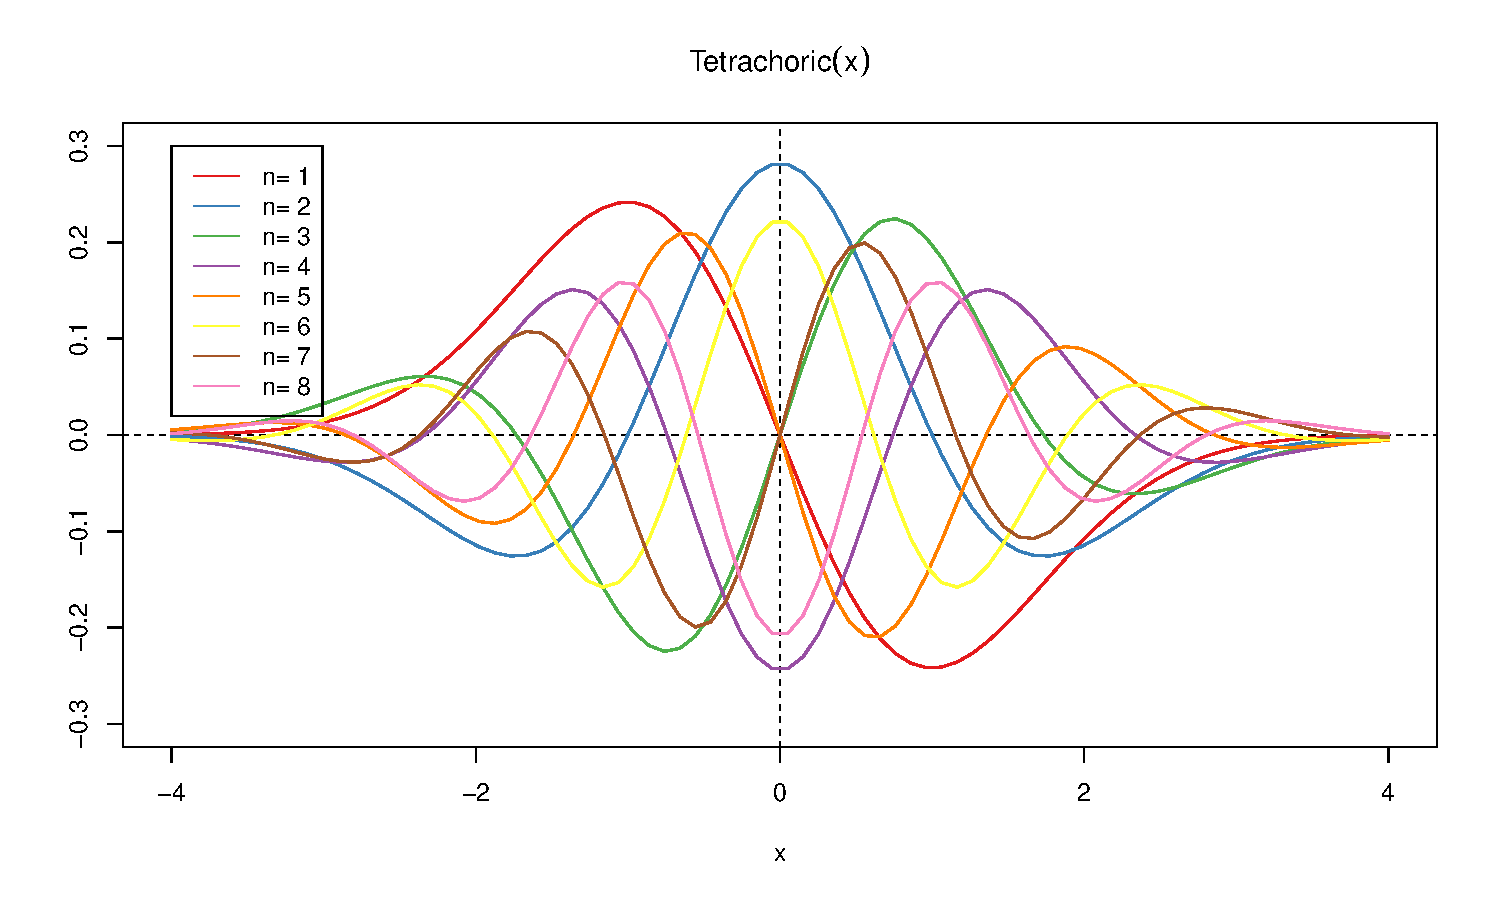
\includegraphics[width=.8\textwidth,height=.4\textwidth]{figure/Tetrachoric.pdf}
  \caption{Tetrachoric函数}
\end{figure} 

\section{符号计算扩展包}
\subsection{Ryacas}
想要做更多的符号计算内容,如解方程,泰勒展开等,可以借助第三方R扩展包Ryacas \cite{Ryacas}

\begin{knitrout}
\definecolor{shadecolor}{rgb}{0.973, 0.973, 0.973}\color{fgcolor}\begin{kframe}
\begin{alltt}
\hlkwd{suppressPackageStartupMessages}\hlstd{(}\hlkwd{library}\hlstd{(Ryacas))}
\hlkwd{yacas}\hlstd{(}\hlstr{"Solve(x/(1+x) == a, x)"}\hlstd{)}
\end{alltt}
\begin{verbatim}
## expression(list(x == a/(1 - a)))
\end{verbatim}
\begin{alltt}
\hlkwd{yacas}\hlstd{(}\hlkwd{expression}\hlstd{(}\hlkwd{Expand}\hlstd{((}\hlnum{1}\hlopt{+}\hlstd{x)}\hlopt{^}\hlnum{3}\hlstd{)))}
\end{alltt}
\begin{verbatim}
## expression(x^3 + 3 * x^2 + 3 * x + 1)
\end{verbatim}
\begin{alltt}
\hlkwd{yacas}\hlstd{(}\hlstr{"OdeSolve(y''==4*y)"}\hlstd{)}
\end{alltt}
\begin{verbatim}
## expression(C110 * exp(2 * x) + C114 * exp(-2 * x))
\end{verbatim}
\begin{alltt}
\hlkwd{yacas}\hlstd{(}\hlstr{"Taylor(x,a,3) Exp(x)"}\hlstd{)}
\end{alltt}
\begin{verbatim}
## expression(exp(a) + exp(a) * (x - a) + (x - a)^2 * exp(a)/2 + 
##     (x - a)^3 * exp(a)/6)
\end{verbatim}
\end{kframe}
\end{knitrout}


\subsection{rSymPy}

rSymPy是Python的符号计算库SymPy的R接口

\begin{knitrout}
\definecolor{shadecolor}{rgb}{0.973, 0.973, 0.973}\color{fgcolor}\begin{kframe}
\begin{alltt}
\hlkwd{library}\hlstd{(rSymPy)}
\end{alltt}


{\ttfamily\noindent\itshape\color{messagecolor}{\#\# Loading required package: rJython}}

{\ttfamily\noindent\itshape\color{messagecolor}{\#\# Loading required package: rJava}}

{\ttfamily\noindent\itshape\color{messagecolor}{\#\# Loading required package: rjson}}

{\ttfamily\noindent\itshape\color{messagecolor}{\#\# \\\#\# Attaching package: 'rSymPy'}}

{\ttfamily\noindent\itshape\color{messagecolor}{\#\# The following objects are masked from 'package:Ryacas':\\\#\# \\\#\#\ \ \ \  as.character.Sym, deriv.Sym, Integrate, Limit, List, Math.Sym,\\\#\#\ \ \ \  Ops.Sym, print.Sym, Sym}}\begin{alltt}
\hlstd{x} \hlkwb{<-} \hlkwd{Var}\hlstd{(}\hlstr{"x"}\hlstd{)}
\hlstd{x}\hlopt{+}\hlstd{x}
\end{alltt}
\begin{verbatim}
## [1] "2*x"
\end{verbatim}
\begin{alltt}
\hlkwd{sympy}\hlstd{(}\hlstr{"y = x*x"}\hlstd{)}
\end{alltt}
\begin{verbatim}
## [1] "x**2"
\end{verbatim}
\begin{alltt}
\hlkwd{sympy}\hlstd{(}\hlstr{"y"}\hlstd{)}
\end{alltt}
\begin{verbatim}
## [1] "x**2"
\end{verbatim}
\begin{alltt}
\hlkwd{sympy}\hlstd{(}\hlstr{"limit(1/x, x, oo)"}\hlstd{)}
\end{alltt}
\begin{verbatim}
## [1] "0"
\end{verbatim}
\begin{alltt}
\hlkwd{sympy}\hlstd{(}\hlstr{"diff(sin(2*x), x, 1)"}\hlstd{)}
\end{alltt}
\begin{verbatim}
## [1] "2*cos(2*x)"
\end{verbatim}
\begin{alltt}
\hlkwd{sympy}\hlstd{(}\hlstr{"diff(sin(2*x), x, 5)"}\hlstd{)}
\end{alltt}
\begin{verbatim}
## [1] "32*cos(2*x)"
\end{verbatim}
\begin{alltt}
\hlkwd{sympy}\hlstd{(}\hlstr{"integrate(exp(-x), (x, 0, oo))"}\hlstd{)}
\end{alltt}
\begin{verbatim}
## [1] "1"
\end{verbatim}
\begin{alltt}
\hlkwd{cat}\hlstd{(}\hlkwd{sympy}\hlstd{(}\hlstr{"A = Matrix([[1,x], [y,1]])"}\hlstd{),} \hlstr{"\textbackslash{}n"}\hlstd{)}
\end{alltt}
\begin{verbatim}
## [   1, x]
## [x**2, 1]
\end{verbatim}
\begin{alltt}
\hlkwd{cat}\hlstd{(}\hlkwd{sympy}\hlstd{(}\hlstr{"A**2"}\hlstd{),} \hlstr{"\textbackslash{}n"}\hlstd{)}
\end{alltt}
\begin{verbatim}
## [1 + x**3,      2*x]
## [  2*x**2, 1 + x**3]
\end{verbatim}
\end{kframe}
\end{knitrout}



\section{符号计算在优化算法中的应用}

学过运筹学或者数值分析课程的可能知道,有不少优化算法是要求导或者求梯度的,
如拟牛顿算法,最速下降法和共轭梯度法,还有求解非线性方程组的拟牛顿算法及其修正算法。\\
下面以求Rosenbrock函数的极小值为例:\\
\begin{figure}[htb]
  \centering
    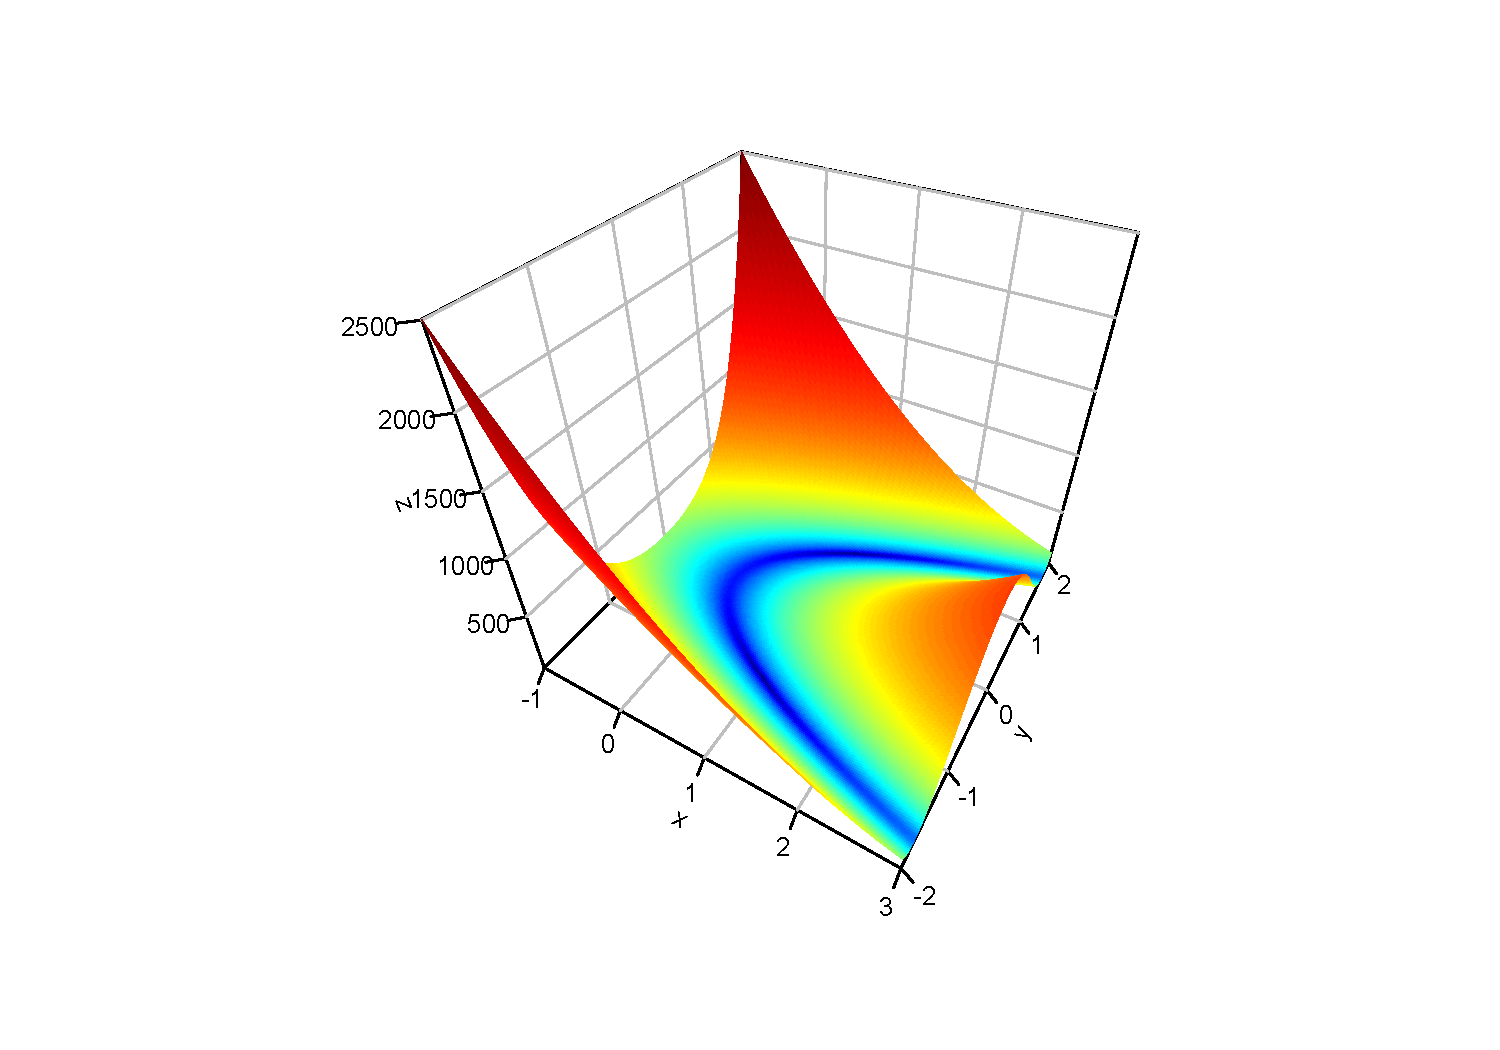
\includegraphics[width=.5\textwidth,height=.5\textwidth]{figure/Rosenbrock.pdf}
  \caption{Rosenbrock函数}
\end{figure}

符号微分

\begin{knitrout}
\definecolor{shadecolor}{rgb}{0.973, 0.973, 0.973}\color{fgcolor}\begin{kframe}
\begin{alltt}
\hlstd{fun}\hlkwb{<-}\hlkwd{expression}\hlstd{(}\hlnum{100}\hlopt{*}\hlstd{(x2}\hlopt{-}\hlstd{x1}\hlopt{^}\hlnum{2}\hlstd{)}\hlopt{^}\hlnum{2}\hlopt{+}\hlstd{(}\hlnum{1}\hlopt{-}\hlstd{x1)}\hlopt{^}\hlnum{2}\hlstd{)}
\hlkwd{D}\hlstd{(fun,}\hlstr{"x1"}\hlstd{)}
\end{alltt}
\begin{verbatim}
## -(2 * (1 - x1) + 100 * (2 * (2 * x1 * (x2 - x1^2))))
\end{verbatim}
\begin{alltt}
\hlkwd{D}\hlstd{(fun,}\hlstr{"x2"}\hlstd{)}
\end{alltt}
\begin{verbatim}
## 100 * (2 * (x2 - x1^2))
\end{verbatim}
\end{kframe}
\end{knitrout}

调用拟牛顿法求极值

\begin{knitrout}
\definecolor{shadecolor}{rgb}{0.973, 0.973, 0.973}\color{fgcolor}\begin{kframe}
\begin{alltt}
\hlstd{fr} \hlkwb{<-} \hlkwa{function}\hlstd{(}\hlkwc{x}\hlstd{) \{}
    \hlstd{x1} \hlkwb{<-} \hlstd{x[}\hlnum{1}\hlstd{]}
    \hlstd{x2} \hlkwb{<-} \hlstd{x[}\hlnum{2}\hlstd{]}
    \hlnum{100} \hlopt{*} \hlstd{(x2} \hlopt{-} \hlstd{x1} \hlopt{*} \hlstd{x1)}\hlopt{^}\hlnum{2} \hlopt{+} \hlstd{(}\hlnum{1} \hlopt{-} \hlstd{x1)}\hlopt{^}\hlnum{2}
\hlstd{\}}
\hlstd{grr1} \hlkwb{<-} \hlkwa{function}\hlstd{(}\hlkwc{x}\hlstd{) \{}
    \hlstd{x1} \hlkwb{<-} \hlstd{x[}\hlnum{1}\hlstd{]}
    \hlstd{x2} \hlkwb{<-} \hlstd{x[}\hlnum{2}\hlstd{]}
    \hlkwd{c}\hlstd{(}\hlopt{-}\hlnum{400} \hlopt{*} \hlstd{x1} \hlopt{*} \hlstd{(x2} \hlopt{-} \hlstd{x1} \hlopt{*} \hlstd{x1)} \hlopt{-} \hlnum{2} \hlopt{*} \hlstd{(}\hlnum{1} \hlopt{-} \hlstd{x1),}
       \hlnum{200} \hlopt{*}      \hlstd{(x2} \hlopt{-} \hlstd{x1} \hlopt{*} \hlstd{x1))}
\hlstd{\}}
\hlkwd{optim}\hlstd{(}\hlkwd{c}\hlstd{(}\hlopt{-}\hlnum{1.2}\hlstd{,}\hlnum{1}\hlstd{), fr, grr1,} \hlkwc{method} \hlstd{=} \hlstr{"BFGS"}\hlstd{)}
\end{alltt}
\begin{verbatim}
## $par
## [1] 1 1
## 
## $value
## [1] 9.594956e-18
## 
## $counts
## function gradient 
##      110       43 
## 
## $convergence
## [1] 0
## 
## $message
## NULL
\end{verbatim}
\end{kframe}
\end{knitrout}

仿照Tetrachoric函数的写法,可以简写grr1函数(这个写法可以稍微避免一点复制粘贴):

\begin{knitrout}
\definecolor{shadecolor}{rgb}{0.973, 0.973, 0.973}\color{fgcolor}\begin{kframe}
\begin{alltt}
\hlstd{grr2}\hlkwb{<-}\hlkwa{function}\hlstd{(}\hlkwc{x}\hlstd{)\{}
  \hlstd{x1} \hlkwb{<-} \hlstd{x[}\hlnum{1}\hlstd{]}
  \hlstd{x2} \hlkwb{<-} \hlstd{x[}\hlnum{2}\hlstd{]}
  \hlkwd{c}\hlstd{(}\hlkwd{eval}\hlstd{(}\hlkwd{D}\hlstd{(fun,}\hlstr{"x1"}\hlstd{)),}\hlkwd{eval}\hlstd{(}\hlkwd{D}\hlstd{(fun,}\hlstr{"x2"}\hlstd{)))}  \hlcom{# 表达式微分}
\hlstd{\}}
\hlkwd{optim}\hlstd{(}\hlkwd{c}\hlstd{(}\hlopt{-}\hlnum{1.2}\hlstd{,}\hlnum{1}\hlstd{), fr, grr2,} \hlkwc{method} \hlstd{=} \hlstr{"BFGS"}\hlstd{)}
\end{alltt}
\begin{verbatim}
## $par
## [1] 1 1
## 
## $value
## [1] 9.594956e-18
## 
## $counts
## function gradient 
##      110       43 
## 
## $convergence
## [1] 0
## 
## $message
## NULL
\end{verbatim}
\end{kframe}
\end{knitrout}

如果调用numDeriv包\cite{numDeriv},可以再少写点代码:

\begin{knitrout}
\definecolor{shadecolor}{rgb}{0.973, 0.973, 0.973}\color{fgcolor}\begin{kframe}
\begin{alltt}
\hlkwd{library}\hlstd{(numDeriv)}
\hlstd{grr3} \hlkwb{<-} \hlkwa{function}\hlstd{(}\hlkwc{x}\hlstd{) \{}
  \hlstd{x1} \hlkwb{<-} \hlstd{x[}\hlnum{1}\hlstd{]}
  \hlstd{x2} \hlkwb{<-} \hlstd{x[}\hlnum{2}\hlstd{]}
  \hlkwd{grad}\hlstd{(fr,}\hlkwd{c}\hlstd{(x1,x2))}  \hlcom{# 函数微分}
\hlstd{\}}
\hlkwd{optim}\hlstd{(}\hlkwd{c}\hlstd{(}\hlopt{-}\hlnum{1.2}\hlstd{,} \hlnum{1}\hlstd{), fr, grr3,} \hlkwc{method} \hlstd{=} \hlstr{"BFGS"}\hlstd{)}
\end{alltt}
\begin{verbatim}
## $par
## [1] 1 1
## 
## $value
## [1] 9.595012e-18
## 
## $counts
## function gradient 
##      110       43 
## 
## $convergence
## [1] 0
## 
## $message
## NULL
\end{verbatim}
\end{kframe}
\end{knitrout}

如果一定要体现符号微分的过程,就调用Deriv包:

\begin{knitrout}
\definecolor{shadecolor}{rgb}{0.973, 0.973, 0.973}\color{fgcolor}\begin{kframe}
\begin{alltt}
\hlkwd{library}\hlstd{(Deriv)}
\hlstd{fr1} \hlkwb{<-} \hlkwa{function}\hlstd{(}\hlkwc{x1}\hlstd{,}\hlkwc{x2}\hlstd{) \{} \hlcom{# 函数形式与上面不同}
  \hlnum{100} \hlopt{*} \hlstd{(x2} \hlopt{-} \hlstd{x1} \hlopt{*} \hlstd{x1)}\hlopt{^}\hlnum{2} \hlopt{+} \hlstd{(}\hlnum{1} \hlopt{-} \hlstd{x1)}\hlopt{^}\hlnum{2}
\hlstd{\}}

\hlstd{grr2} \hlkwb{<-} \hlkwa{function}\hlstd{(}\hlkwc{x}\hlstd{) \{}
  \hlstd{x1} \hlkwb{<-} \hlstd{x[}\hlnum{1}\hlstd{]}
  \hlstd{x2} \hlkwb{<-} \hlstd{x[}\hlnum{2}\hlstd{]}
  \hlkwd{Deriv}\hlstd{(fr1,}\hlkwc{cache.exp} \hlstd{=} \hlnum{FALSE}\hlstd{)(x1,x2)} \hlcom{# 符号微分}
\hlstd{\}}
\hlkwd{optim}\hlstd{(}\hlkwd{c}\hlstd{(}\hlopt{-}\hlnum{1.2}\hlstd{,} \hlnum{1}\hlstd{), fr, grr2,} \hlkwc{method} \hlstd{=} \hlstr{"BFGS"}\hlstd{)}
\end{alltt}
\begin{verbatim}
## $par
## [1] 1 1
## 
## $value
## [1] 9.594956e-18
## 
## $counts
## function gradient 
##      110       43 
## 
## $convergence
## [1] 0
## 
## $message
## NULL
\end{verbatim}
\end{kframe}
\end{knitrout}
从上面可以看出函数(Deriv与optim)之间不兼容:Deriv与optim接受的函数形式不同,导致两个函数(fr与fr1)的参数列表的形式不一样,应能看出fr这种写法更好些。
\\
注:
\begin{enumerate}
  \item 求极值和求解方程(组)往往有联系的,如统计中求参数的最大似然估计,有不少可以转化为求方程(组),如stat4包\cite{R-core}的mle函数。  
  \item 目标函数可以求导,使用拟牛顿算法效果比较好,如上例中methods参数设置成CG,结果就会不一样。
  \item nlm、optim和nlminb等函数都实现了带梯度的优化算法。
  \item 不过话又说回来,真实的场景大多是目标函数不能求导,一阶导数都不能求,更多细节请读者参见optim函数帮助。
  \item 还有一些做数值优化的R包,如BB包\cite{BB}求解大规模非线性系统,numDeriv包是数值微分的通用求解器,更多的内容可参见https://cran.rstudio.com/web/views/Optimization.html。
  \item 除了数值优化还有做概率优化的R包,如仅遗传算法就有GA \cite{R-GA}, gafit \cite{R-gafit},galts \cite{R-galts}, mcga \cite{R-mcga}, rgenoud \cite{R-rgenoud},gaoptim \cite{R-gaoptim}, genalg \cite{R-genalg}等R包,这方面的最新成果参考文献 \cite{2016arXiv160501931S}。
\end{enumerate}


\section{R软件信息}

\begin{knitrout}
\definecolor{shadecolor}{rgb}{0.973, 0.973, 0.973}\color{fgcolor}\begin{kframe}
\begin{alltt}
\hlkwd{sessionInfo}\hlstd{()}
\end{alltt}
\begin{verbatim}
## R version 3.4.3 (2017-11-30)
## Platform: x86_64-pc-linux-gnu (64-bit)
## Running under: Ubuntu 16.04.4 LTS
## 
## Matrix products: default
## BLAS: /usr/lib/openblas-base/libblas.so.3
## LAPACK: /usr/lib/libopenblasp-r0.2.18.so
## 
## locale:
##  [1] LC_CTYPE=en_US.UTF-8          LC_NUMERIC=C                 
##  [3] LC_TIME=en_US.UTF-8           LC_COLLATE=en_US.UTF-8       
##  [5] LC_MONETARY=en_US.UTF-8       LC_MESSAGES=en_US.UTF-8      
##  [7] LC_PAPER=en_US.UTF-8          LC_NAME=en_US.UTF-8          
##  [9] LC_ADDRESS=en_US.UTF-8        LC_TELEPHONE=en_US.UTF-8     
## [11] LC_MEASUREMENT=en_US.UTF-8    LC_IDENTIFICATION=en_US.UTF-8
## 
## attached base packages:
## [1] stats     graphics  grDevices utils     datasets  methods   base     
## 
## other attached packages:
## [1] numDeriv_2016.8-1 rSymPy_0.2-1.1    rJython_0.0-4     rjson_0.2.15     
## [5] rJava_0.9-9       Ryacas_0.3-1      Deriv_3.8.4       knitr_1.20       
## 
## loaded via a namespace (and not attached):
## [1] compiler_3.4.3  magrittr_1.5    tools_3.4.3     Rcpp_0.12.15   
## [5] stringi_1.1.6   highr_0.6       stringr_1.3.0   XML_3.98-1.10  
## [9] evaluate_0.10.1
\end{verbatim}
\end{kframe}
\end{knitrout}

本文是在RStudio环境下用R sweave编写的,用knitr\cite{R-knitr}处理R代码,\XeLaTeX{}编译生成pdf文档。 编译之前安装必要的R包

\begin{knitrout}
\definecolor{shadecolor}{rgb}{0.973, 0.973, 0.973}\color{fgcolor}\begin{kframe}
\begin{alltt}
\hlstd{Pkgs} \hlkwb{<-} \hlkwd{c}\hlstd{(}\hlstr{"Ryacas"}\hlstd{,}\hlstr{"numDeriv"}\hlstd{,}\hlstr{"Deriv"}\hlstd{,}\hlstr{"knitr"}\hlstd{,}\hlstr{"rSymPy"}\hlstd{)}
\hlkwd{installed.packages}\hlstd{(Pkgs)}
\end{alltt}
\end{kframe}
\end{knitrout}


\renewcommand\refname{参考文献} 
\bibliographystyle{unsrt}
\bibliography{mybib.bib} 




\end{document}
